\documentclass[dvipsnames,14pt,t]{beamer}
\usepackage{slides}
\usepackage{langs}
\usepackage{graph}
\usepackage{soul}
\usepackage{data}
\usepackage{proof}

% beamer stuff 
\renewcommand{\slidecaption}{Canterbury, 22.2.2016}
\newcommand{\bl}[1]{\textcolor{blue}{#1}}

\begin{document}
%%%%%%%%%%%%%%%%%%%%%%%%%%%%%%%%%%%%%%%%%%%%%%%%%%%%%%%%%%%%%%%%%
\begin{frame}[t]
\frametitle{%
  \begin{tabular}{@ {}c@ {}}
  \\
  \Large POSIX Lexing with Derivatives\\[-1.5mm] 
  \Large of Regular Expressions\\[-1mm] 
  %\normalsize Or, How to Find Bugs with the\\[-5mm] 
  %\normalsize Isabelle Theorem Prover
  \end{tabular}}\bigskip\bigskip\bigskip

  \normalsize
  \begin{center}
  \begin{tabular}{c}
  \small Christian Urban\\
  \small King's College London\\
  \\
  \\
  Joint work with Fahad Ausaf and Roy Dyckhoff
  \end{tabular}
  \end{center}

\end{frame}
%%%%%%%%%%%%%%%%%%%%%%%%%%%%%%%%%%%%%%%%%%%%%%%%%%%%%%%%%%%%%%%%%%     

%%%%%%%%%%%%%%%%%%%%%%%%%%%%%%%%%%%%%%%%%%%%%%%%%%%%%%%%%%%
  \begin{frame}[c]

  \begin{center}
  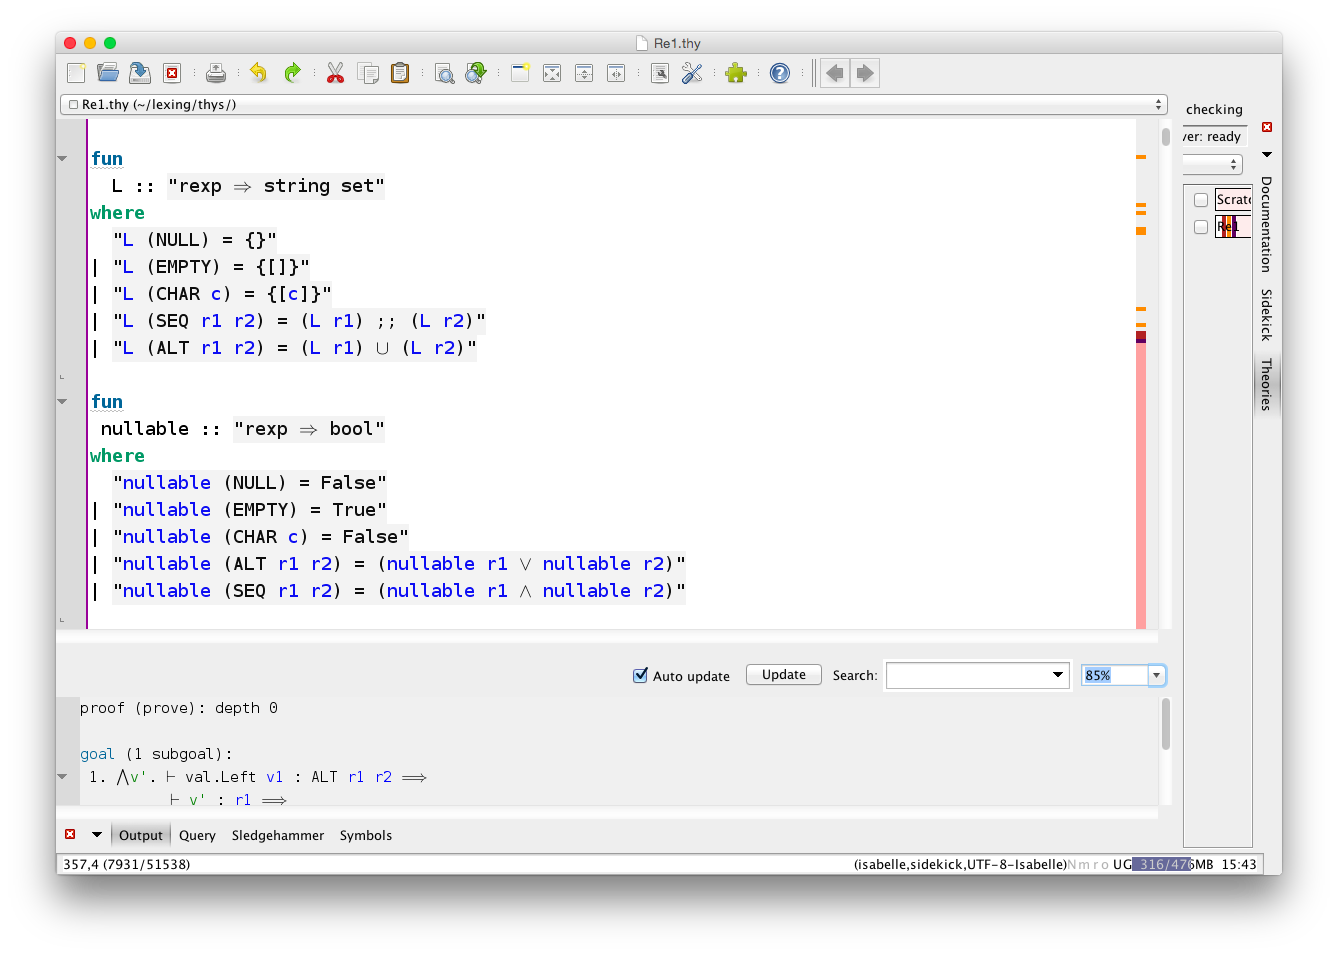
\includegraphics[scale=0.2]{pics/isabelle.png}
  \end{center}
  \mbox{}\\[-20mm]\mbox{}

  \begin{itemize}
  \item Isabelle interactive theorem prover; 
  some proofs are automatic -- most however need help
  \item the learning curve is steep; you often have to fight the 
  theorem prover\ldots no different in other ITPs
  \end{itemize}

  \end{frame}
%%%%%%%%%%%%%%%%%%%%%%%%%%%%%%%%%%%%%%%%%%%%%%%%%%%%%%%%%%%

%%%%%%%%%%%%%%%%%%%%%%%%%%%%%%%%%%%%%%%%%%%%%%%%%%%%%%%%%%%%%%%%%%
\begin{frame}[c]
\frametitle{Why Bother?}

Surely regular expressions must have been implemented and 
studied to death, no?

\begin{center}
\begin{tikzpicture}
\begin{axis}[
    xlabel={{\tt a}s},
    ylabel={time in secs},
    enlargelimits=false,
    xtick={0,5,...,30},
    xmax=30,
    ymax=35,
    ytick={0,5,...,30},
    scaled ticks=false,
    axis lines=left,
    width=8cm,
    height=6cm, 
    legend entries={Python,Ruby},  
    legend pos=north west,
    legend cell align=left  
]
\addplot[blue,mark=*, mark options={fill=white}] 
  table {data/re-python.data};
\addplot[brown,mark=pentagon*, mark options={fill=white}] 
  table {data/re-ruby.data};  
\end{axis}
\end{tikzpicture}
\end{center}

evil regular expressions: \bl{$({\tt a}?)^n \cdot {\tt a}^n$}

\end{frame}
%%%%%%%%%%%%%%%%%%%%%%%%%%%%%%%%%%%%%%%%%%%%%%%%%%%%%%%%%%%%%%%%%%   


%%%%%%%%%%%%%%%%%%%%%%%%%%%%%%%%%%%%%%%%%%%%%%%%%%%%%%%%%%%%%%%%%%
\begin{frame}[c]
\frametitle{\Large Isabelle Theorem Prover}

\begin{itemize}
\item started to use Isabelle after my PhD (in 2000)

\item the thesis included a rather complicated 
  ``pencil-and-paper'' proof for a 
  termination argument (sort of $\lambda$-calculus)\medskip
 
\item me, my supervisor, the examiners did not find any problems\medskip 
 \begin{center}
  \begin{tabular}{@ {}c@ {}}
  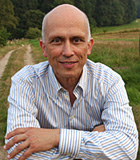
\includegraphics[scale=0.38]{pics/barendregt.jpg}\\[-2mm]
  \footnotesize Henk Barendregt
  \end{tabular}
  \hspace{2mm}
  \begin{tabular}{@ {}c@ {}}
  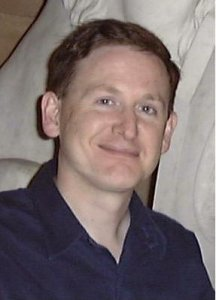
\includegraphics[scale=0.20]{pics/andrewpitts.jpg}\\[-2mm]
  \footnotesize Andrew Pitts
  \end{tabular}
  \end{center}
  
\item people were building their work on my result      
  
\end{itemize}

\end{frame}
%%%%%%%%%%%%%%%%%%%%%%%%%%%%%%%%%%%%%%%%%%%%%%%%%%%%%%%%%%%%%%%%%%  

%%%%%%%%%%%%%%%%%%%%%%%%%%%%%%%%%%%%%%%%%%%%%%%%%%%%%%%%%%%%%%%%%%
\begin{frame}[t]
\frametitle{\Large Nominal Isabelle}

\begin{itemize}
\item implemented a package for the Isabelle prover 
in order to reason conveniently about binders 
 
\begin{center}
\large\bl{$\lambda \alert{x}.\,M$} \hspace{10mm}
\bl{$\forall \alert{x}.\,P\,x$}
\end{center}\bigskip\bigskip\bigskip\bigskip
\bigskip\bigskip\bigskip\pause\pause
  
  
\item when finally being able to formalise the proof from my PhD, I found that the main result
      (termination) is correct, but a central lemma needed to
      be generalised
\end{itemize}

\only<2->{
\begin{textblock}{3}(13,5)

\includegraphics[scale=0.33]{pics/skeleton.jpg}
\end{textblock}}

\begin{textblock}{3}(5.3,7)
\onslide<1->{
\begin{tikzpicture}
\node at (0,0) [single arrow, shape border rotate=90, fill=red,text=red]{\mbox{a}};
\end{tikzpicture}}
\end{textblock}

\begin{textblock}{3}(8.7,7)
\onslide<1->{
\begin{tikzpicture}
\node at (0,0) [single arrow, shape border rotate=90, fill=red,text=red]{\mbox{a}};
\end{tikzpicture}}
\end{textblock}

\end{frame}
%%%%%%%%%%%%%%%%%%%%%%%%%%%%%%%%%%%%%%%%%%%%%%%%%%%%%%%%%%%%%%%%%%  


%%%%%%%%%%%%%%%%%%%%%%%%%%%%%%%%%%%%%%%%%%%%%%%%%%%%%%%%%%%%%%%%%%
\begin{frame}[c]
\frametitle{\Large Variable Convention}


\begin{center}
\begin{bubble}[10cm]
  \color{gray}  
  \small
  {\bf\mbox{}Variable Convention:}\\[1mm] 
  If $M_1,\ldots,M_n$ occur in a certain mathematical context
  (e.g. definition, proof), then in these terms all bound variables 
  are chosen to be different from the free variables.\\[2mm]
  
  \footnotesize\hfill Barendregt in ``The Lambda-Calculus: Its Syntax and Semantics''
\end{bubble}
\end{center}

\mbox{}\\[-8mm]
\begin{itemize}


\item instead of proving a property for \alert{\bf all} bound
variables, you prove it only for \alert{\bf some}\ldots?

\item feels like it is used in 90\% of papers in PT and FP
(9.9\% use de-Bruijn indices)

\item this is mostly OK, but in some corner-cases you can use it
to prove \alert{\bf false}\ldots we fixed this!
\end{itemize}

\end{frame}
%%%%%%%%%%%%%%%%%%%%%%%%%%%%%%%%%%%%%%%%%%%%%%%%%%%%%%%%%%%%%%%%%%  

%%%%%%%%%%%%%%%%%%%%%%%%%%%%%%%%%%%%%%%%%%%%%%%%%%%%%%%%%%%%%%%%%%  
\begin{frame}[c]
\frametitle{}

\begin{tabular}{c@ {\hspace{2mm}}c}
\\[6mm]
\begin{tabular}{c}
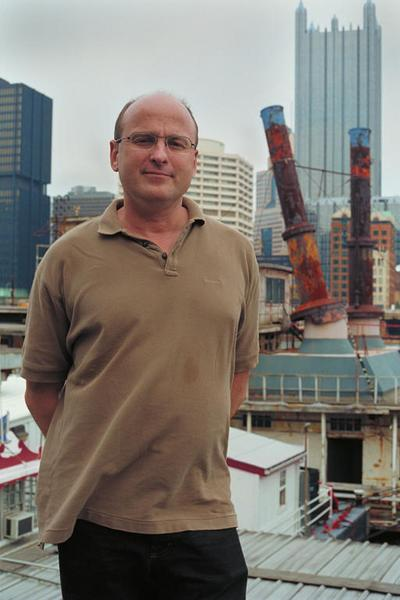
\includegraphics[scale=0.11]{pics/harper.jpg}\\[-2mm]
{\footnotesize Bob Harper}\\[-2mm]
{\footnotesize}
\end{tabular}
\begin{tabular}{c}
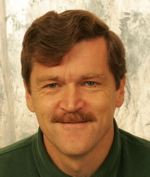
\includegraphics[scale=0.37]{pics/pfenning.jpg}\\[-2mm]
{\footnotesize Frank Pfenning}\\[-2mm]
{\footnotesize}
\end{tabular} &

\begin{tabular}{p{6cm}}
\raggedright
{published a proof in\\ {\bf ACM Transactions on Computational Logic}, 2005,
$\sim$31pp}
\end{tabular}\\

\\[0mm]
  
\begin{tabular}{c}
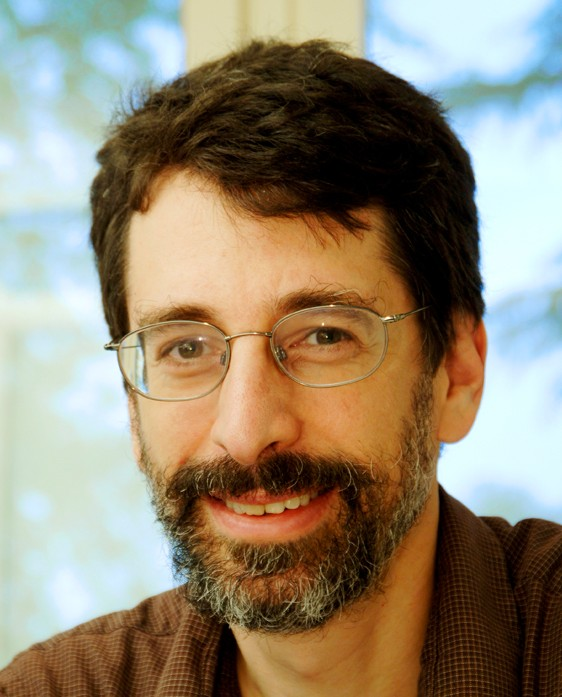
\includegraphics[scale=0.36]{pics/appel.jpg}\\[-2mm] 
{\footnotesize Andrew Appel}\\[-2.5mm]
{\footnotesize}
\end{tabular} &

\begin{tabular}{p{6cm}}
\raggedright
{relied on their proof in a\\ {\bf security} critical application}
\end{tabular}
\end{tabular}

\end{frame}
%%%%%%%%%%%%%%%%%%%%%%%%%%%%%%%%%%%%%%%%%%%%%%%%%%%%%%%%%%%%%%%%%%

%%%%%%%%%%%%%%%%%%%%%%%%%%%%%%%%%%%%%%%%%%%%%%%%%%%%%%%%%%%%%%%%%%
\begin{frame}
\frametitle{Proof-Carrying Code}

\begin{textblock}{10}(2.5,2.2)
\begin{block}{Idea:}
\begin{center}
\begin{tikzpicture}
\draw[help lines,cream] (0,0.2) grid (8,4);
  
\draw[line width=1mm, red] (5.5,0.6) rectangle (7.5,4);
\node[anchor=base] at (6.5,2.8) 
     {\small\begin{tabular}{@ {}p{1.9cm}@ {}}\centering  user: untrusted code\end{tabular}};

\draw[line width=1mm, red] (0.1,0.6) rectangle (2.1,4);
  \node[anchor=base] at (1.1,2.3) 
     {\small\begin{tabular}{@ {}p{1.9cm}@ {}}\centering  developer ---\\ web server\end{tabular}};
  
\onslide<3->{
  \draw[line width=1mm, red, fill=red] (5.5,0.6) rectangle (7.5,1.8);
  \node[anchor=base,white] at (6.5,1.1) 
     {\small\begin{tabular}{@ {}p{1.9cm}@ {}}\bf\centering proof- checker\end{tabular}};}

  \node at (3.6,3.0) [single arrow, fill=red,text=white, 
                      minimum height=3.4cm]{\bf code};
  \onslide<2->{
  \node at (3.6,1.3) [single arrow, fill=red,text=white, 
                      minimum height=3.4cm]{\bf certificate};
  \node at (3.6,1.9) {\small\color{gray}{\mbox{}\hspace{-1mm}a proof in LF}};
}

  
\end{tikzpicture}
\end{center}
\end{block}
\end{textblock}

\begin{textblock}{15}(2,12)
\small
\begin{itemize}
\item<3-> Appel's checker is $\sim$2700 lines of code (1865 loc of\\ LF definitions; 
803 loc in C including 2 library functions)\\[-3mm]
\item<3-> 167 loc in C implement a type-checker
\end{itemize}
\end{textblock}

\end{frame}
%%%%%%%%%%%%%%%%%%%%%%%%%%%%%%%%%%%%%%%%%%%%%%%%%%%%%%%%%%%%%%%%%%

%%%%%%%%%%%%%%%%%%%%%%%%%%%%%%%%%%%%%%%%%%%%%%%%%%%%%%%%%%%%%%%%%%
  \begin{frame}<2->[squeeze]
  \frametitle{} 
  
  \begin{columns}
  \tikzstyle{every node}=[node distance=25mm,text height=1.5ex, text depth=.25ex]
  \tikzstyle{node1}=[rectangle, minimum size=10mm, rounded corners=3mm, very thick, 
                     draw=black!50, top color=white, bottom color=black!20]
  \tikzstyle{node2}=[rectangle, minimum size=12mm, rounded corners=3mm, very thick, 
                     draw=red!70, top color=white, bottom color=red!50!black!20]
  
  \begin{column}{0.8\textwidth}
  \begin{textblock}{0}(1,2)

  \begin{tikzpicture}
  \matrix[ampersand replacement=\&,column sep=7mm, row sep=5mm]
  { \&[-10mm] 
    \node (def1)   [node1] {\large\hspace{1mm}Spec\hspace{1mm}\mbox{}}; \&
    \node (proof1) [node1] {\large Proof}; \&
    \node (alg1)   [node1] {\large\hspace{1mm}Alg\hspace{1mm}\mbox{}}; \\
    
    \onslide<4->{\node {\begin{tabular}{c}\small 1st\\[-2.5mm] \footnotesize solution\end{tabular}};} \&
    \onslide<4->{\node (def2)   [node2] {\large Spec$^\text{+ex}$};} \&
    \onslide<4->{\node (proof2) [node1] {\large Proof};} \&
    \onslide<4->{\node (alg2)   [node1] {\large\hspace{1mm}Alg\hspace{1mm}\mbox{}};} \\
     
    \onslide<5->{\node {\begin{tabular}{c}\small 2nd\\[-2.5mm] \footnotesize solution\end{tabular}};} \&
    \onslide<5->{\node (def3)   [node1] {\large\hspace{1mm}Spec\hspace{1mm}\mbox{}};} \&
    \onslide<5->{\node (proof3) [node1] {\large Proof};} \&
    \onslide<5->{\node (alg3)   [node2] {\large Alg$^\text{-ex}$};} \\

    \onslide<6->{\node {\begin{tabular}{c}\small 3rd\\[-2.5mm] \footnotesize solution\end{tabular}};} \&
    \onslide<6->{\node (def4)   [node1] {\large\hspace{1mm}Spec\hspace{1mm}\mbox{}};} \&
    \onslide<6->{\node (proof4) [node2] {\large\hspace{1mm}Proof\hspace{1mm}};} \&
    \onslide<6->{\node (alg4)   [node1] {\large\hspace{1mm}Alg\hspace{1mm}\mbox{}};} \\
  };

  \draw[->,black!50,line width=2mm] (proof1) -- (def1);
  \draw[->,black!50,line width=2mm] (proof1) -- (alg1);
  
  \onslide<4->{\draw[->,black!50,line width=2mm] (proof2) -- (def2);}
  \onslide<4->{\draw[->,black!50,line width=2mm] (proof2) -- (alg2);}

  \onslide<5->{\draw[->,black!50,line width=2mm] (proof3) -- (def3);}
  \onslide<5->{\draw[->,black!50,line width=2mm] (proof3) -- (alg3);}
  
  \onslide<6->{\draw[->,black!50,line width=2mm] (proof4) -- (def4);}
  \onslide<6->{\draw[->,black!50,line width=2mm] (proof4) -- (alg4);}

  \onslide<3->{\draw[white,line width=1mm] (1.1,3.2) -- (0.9,2.85) -- (1.1,2.35) -- (0.9,2.0);} 
  \end{tikzpicture}

  \end{textblock}
  \end{column}
  \end{columns}


  \begin{textblock}{3}(12,3.6)
  \onslide<4->{
  \begin{tikzpicture}
  \node at (0,0) [single arrow, shape border rotate=270, fill=red,text=white]{2h};
  \end{tikzpicture}}
  \end{textblock}
  
  \begin{textblock}{0}(0.4,12.8)
  \onslide<6->{
  \begin{bubble}[11cm]
  \small Each time one needs to check $\sim$31pp~of 
  informal paper proofs.
  You have to be able to keep definitions 
  and proofs consistent.
  \end{bubble}}
  \end{textblock}

  \end{frame}
%%%%%%%%%%%%%%%%%%%%%%%%%%%%%%%%%%%%%%%%%%%%%%%%%%%%%%%%%%%%%%%%%%     

%%%%%%%%%%%%%%%%%%%%%%%%%%%%%%%%%%%%%%%%%%%%%%%%%%%%%%%%%%%%%%%%%%
%  \begin{frame}[c]
%  \frametitle{\Large Lessons Learned}
%
%  \begin{itemize}
%  \item using a theorem prover we were able to keep a large 
%  proof consistent with changes in the definitions\bigskip
%  \item it took us some 10 days to get to the error\ldots
%  probably the same time Harper and Pfenning needed to \LaTeX{}
%  their paper\bigskip 
%  \item once there, we ran circles around them
%  \end{itemize}
%
%  \end{frame}
%%%%%%%%%%%%%%%%%%%%%%%%%%%%%%%%%%%%%%%%%%%%%%%%%%%%%%%%%%%%%%%%%%  
  

%%%%%%%%%%%%%%%%%%%%%%%%%%%%%%%%%%%%%%%%%%%%%%%%%%%%%%%%%%%%%%%%%%
  \begin{frame}[c]
  \frametitle{Real-Time Scheduling} 

  \begin{textblock}{11}(1,3)
  \begin{tabular}{@{\hspace{-10mm}}l}
  \begin{tikzpicture}[scale=1.1]
  \node at (-2.5,-1.5) {\textcolor{white}{a}};
  \node at (8,4) {\textcolor{white}{a}};
  
    
  \only<1>{
   \draw[fill, blue!50] (1,0) rectangle (3,0.6);
  }
  \only<2>{
   \draw[fill, blue!50] (1,0) rectangle (2,0.6);
   \draw[fill, blue!50] (3,0) rectangle (5,0.6);
   \draw[fill, blue!100] (2,3) rectangle (3,3.6);
  }
  \only<3>{
   \draw[fill, blue!50] (1,0) rectangle (2,0.6);
   \draw[fill, blue!50] (3,0) rectangle (4.5,0.6);
   \draw[fill, blue!50] (5.5,0) rectangle (6,0.6);
   \draw[fill, blue!100] (2,3) rectangle (3,3.6);
   \draw[fill, blue!100] (4.5,3) rectangle (5.5,3.6);
  }
  \only<4>{
   \node at (2.5,0.9) {\small locks a resource};
   \draw[fill, blue!50] (1,0) rectangle (2,0.6);
   \draw[blue!50, very thick] (2,0) rectangle (4,0.6);
   \draw[blue!100, very thick] (2,3) rectangle (3, 3.6);
   \draw[red, <-, line width = 2mm] (2,-0.1) -- (2, -1);
  }
  \only<5>{
   \node at (2.5,0.9) {\small locks a resource};
   \draw[fill, blue!50] (1,0) rectangle (4,0.6);
   \draw[blue!100, fill] (4,3) rectangle (5, 3.6);
  }
  \only<6>{
   \node at (2.5,0.9) {\small locks a resource};
   \draw[fill, blue!50] (1,0) rectangle (2,0.6);
   \draw[blue!50, very thick] (2,0) rectangle (4,0.6);
   \draw[blue!100, very thick] (2,3) rectangle (3, 3.6);
   \draw[red, <-, line width = 2mm] (2,-0.1) -- (2, -1);
  }
  \only<7>{
   \node at (2.5,0.9) {\small locks a resource};
   \draw[fill, blue!50] (1,0) rectangle (2.5,0.6);
   \draw[blue!50, very thick] (2.5,0) rectangle (4,0.6);
   \draw[blue!100, very thick] (2.5,3) rectangle (3.5, 3.6);
   \draw[red, <-, line width = 2mm] (2.5,-0.1) -- (2.5, -1);
  }
  \only<8>{
   \node at (2.5,0.9) {\small locks a resource}; 
   \draw[fill, blue!50] (1,0) rectangle (2.5,0.6);
   \draw[blue!50, very thick] (2.5,0) rectangle (4,0.6);
   \draw[blue!100, very thick] (2.5,3) rectangle (3.5, 3.6);
   \draw[blue!100, very thick] (2.5,3) rectangle (3.5, 3.6);
   \draw[red, fill] (2.5,1.5) rectangle (3.5,2.1);
   \draw[red, <-, line width = 2mm] (2.5,-0.1) -- (2.5, -1);
  }
  \only<9>{
   \node at (2.5,0.9) {\small locks a resource}; 
   \draw[fill, blue!50] (1,0) rectangle (2.5,0.6);
   \draw[blue!50, very thick] (3.5,0) rectangle (5,0.6);
   \draw[blue!100, very thick] (3.5,3) rectangle (4.5, 3.6);
   \draw[red, fill] (2.5,1.5) rectangle (3.5,2.1);
   \draw[red, <-, line width = 2mm] (3.5,-0.1) -- (3.5, -1);
  }
  \only<10>{
   \node at (2.5,0.9) {\small locks a resource}; 
   \draw[fill, blue!50] (1,0) rectangle (2.5,0.6);
   \draw[blue!50, very thick] (3.5,0) rectangle (5,0.6);
   \draw[blue!100, very thick] (3.5,3) rectangle (4.5, 3.6);
   \draw[red, fill] (2.5,1.5) rectangle (3.5,2.1);
   \draw[red, fill] (3.55,1.5) rectangle (4.5,2.1);
   \draw[red, <-, line width = 2mm] (3.5,-0.1) -- (3.5, -1);
  }
  \only<11>{
   \node at (2.5,0.9) {\small locks a resource};
   \draw[fill, blue!50] (1,0) rectangle (2.5,0.6);
   \draw[blue!50, very thick] (4.5,0) rectangle (6,0.6);
   \draw[blue!100, very thick] (4.5,3) rectangle (5.5, 3.6);
   \draw[red, fill] (2.5,1.5) rectangle (3.5,2.1);
   \draw[red, fill] (3.55,1.5) rectangle (4.5,2.1);
   \draw[red, <-, line width = 2mm] (4.5,-0.1) -- (4.5, -1);
  }
  \only<12>{
   \node at (2.5,0.9) {\small locks a resource}; 
   \draw[fill, blue!50] (1,0) rectangle (2.5,0.6);
   \draw[blue!50, very thick] (5.5,0) rectangle (7,0.6);
   \draw[blue!100, very thick] (5.5,3) rectangle (6.5, 3.6);
   \draw[red, fill] (2.5,1.5) rectangle (3.5,2.1);
   \draw[red, fill] (3.55,1.5) rectangle (4.5,2.1);
   \draw[red, fill] (4.55,1.5) rectangle (5.5,2.1);
   \draw[red, <-, line width = 2mm] (5.5,-0.1) -- (5.5, -1);
   \node [anchor=base] at (6.3, 1.8) {\Large\ldots};
  }
  \only<13>{
   \node at (2.5,0.9) {\small locks a resource}; 
   \draw[fill, blue!50] (1,0) rectangle (2,0.6);
   \draw[blue!50, very thick] (2,0) rectangle (4,0.6);
   \draw[blue!100, very thick] (2,3) rectangle (3, 3.6);
   \draw[red, <-, line width = 2mm] (2,-0.1) -- (2, -1);
  }
  \only<14>{
   \node at (2.5,3.9) {\small locks a resource}; 
   \draw[fill, blue!50] (1,0) rectangle (2,0.6);
   \draw[blue!50, fill] (2,3) rectangle (4,3.6);
   \draw[blue!100, very thick] (4,3) rectangle (5, 3.6);
   \draw[blue!50, ->, line width = 2mm] (2,1) -- (2, 2.5);
   \draw[red, <-, line width = 2mm] (2,-0.1) -- (2, -1);
  }
  \only<15>{
   \node at (2.5,3.9) {\small locks a resource};  
   \draw[fill, blue!50] (1,0) rectangle (2,0.6);
   \draw[blue!50, fill] (2,3) rectangle (4,3.6);
   \draw[blue!100, very thick] (4,3) rectangle (5, 3.6);
   \draw[red, <-, line width = 2mm] (2.5,-0.1) -- (2.5, -1);
   \draw[red, very thick] (2.5,1.5) rectangle (3.5,2.1); 
  }


  \draw[very thick,->](0,0) -- (8,0);
  \node [anchor=base] at (8, -0.3) {\scriptsize time};
  \node [anchor=base] at (0, -0.3) {\scriptsize 0};
  \node [anchor=base] at (-1.2, 0.2) {\small low priority};
  \only<2->{\node [anchor=base] at (-1.2, 3.2) {\small high priority};}
  \only<8->{\node [anchor=base] at (-1.5, 1.7) {\small medium pr.};}

  \end{tikzpicture}
  \end{tabular}
  \end{textblock}

  \begin{textblock}{0}(2.5,13)%
  \small
  \onslide<3->{
  \begin{bubble}[8cm]%
  RT-Scheduling: You want to avoid that a 
  high-priority process is starved indefinitely.
  \end{bubble}}
  \end{textblock}

  \end{frame}
%%%%%%%%%%%%%%%%%%%%%%%%%%%%%%%%%%%%%%%%%%%%%%%%%%%%%%%%%%%%%%%%%%  
  
%%%%%%%%%%%%%%%%%%%%%%%%%%%%%%%%%%%%%%%%%%%%%%%%%%%%%%%%%%%%%%%%%%
  \begin{frame}[c]
  \frametitle{\Large Priority Inheritance Scheduling}

  \begin{itemize}
  \item Let a low priority process \bl{$L$} temporarily inherit 
    the high priority of \bl{$H$} until \bl{$L$} leaves the critical 
    section unlocking the resource.\bigskip
  \item Once the resource is unlocked, \bl{$L$} ``returns to its original 
    priority level.''\\
    \mbox{}\hfill\footnotesize
    \begin{tabular}{p{6cm}@{}}
    L.~Sha, R.~Rajkumar, and J.~P.~Lehoczky. 
    {\it Priority Inheritance Protocols: An Approach to 
    Real-Time Synchronization}. IEEE Transactions on 
    Computers, 39(9):1175–1185, 1990
    \end{tabular}\bigskip\normalsize\pause
  
  \item Proved correct, reviewed in a respectable journal....what could possibly be wrong?
    
  \end{itemize}

  \end{frame}
%%%%%%%%%%%%%%%%%%%%%%%%%%%%%%%%%%%%%%%%%%%%%%%%%%%%%%%%%%%%%%%%%%  
  
%%%%%%%%%%%%%%%%%%%%%%%%%%%%%%%%%%%%%%%%%%%%%%%%%%%%%%%%%%%%%%%%%%
  \begin{frame}[c]

  \begin{textblock}{11}(1,3)
  \begin{tabular}{@{\hspace{-10mm}}l}
  \begin{tikzpicture}[scale=1.1]
  \node at (-2.5,-1.5) {\textcolor{white}{a}};
  \node at (8,4) {\textcolor{white}{a}};
  
  \only<1>{
    \draw[fill, blue!50] (1,0) rectangle (6,0.6);
    \node at (1.5,0.9) {\small $A_L$};
    \node at (2.0,0.9) {\small $B_L$};
    \node at (3.5,0.9) {\small $A_R$};
    \node at (5.7,0.9) {\small $B_R$};
    \draw[very thick,blue!100] (1.5,0) -- (1.5,0.6);
    \draw[very thick,blue!100] (2.0,0) -- (2.0,0.6);
    \draw[very thick,blue!100] (3.5,0) -- (3.5,0.6);
    \draw[very thick,blue!100] (5.7,0) -- (5.7,0.6);
  }
  \only<2>{
    \draw[fill, blue!50] (1,0) rectangle (3,0.6);
    \draw[very thick, blue!50] (3,0) rectangle (6,0.6);
    \node at (1.5,0.9) {\small $A_L$};
    \node at (2.0,0.9) {\small $B_L$};
    \node at (3.5,0.9) {\small $A_R$};
    \node at (5.7,0.9) {\small $B_R$};
    \draw[very thick,blue!100] (1.5,0) -- (1.5,0.6);
    \draw[very thick,blue!100] (2.0,0) -- (2.0,0.6);
    \draw[very thick,blue!100] (3.5,0) -- (3.5,0.6);
    \draw[very thick,blue!100] (5.7,0) -- (5.7,0.6);
  }
  \only<3>{
    \draw[fill, blue!50] (1,0) rectangle (3,0.6);
    \draw[very thick, blue!50] (3,0) rectangle (6,0.6);
    \node at (1.5,0.9) {\small $A_L$};
    \node at (2.0,0.9) {\small $B_L$};
    \node at (3.5,0.9) {\small $A_R$};
    \node at (5.7,0.9) {\small $B_R$};
    \draw[very thick,blue!100] (1.5,0) -- (1.5,0.6);
    \draw[very thick,blue!100] (2.0,0) -- (2.0,0.6);
    \draw[very thick,blue!100] (3.5,0) -- (3.5,0.6);
    \draw[very thick,blue!100] (5.7,0) -- (5.7,0.6);
    \draw[very thick,blue!100] (3,3) rectangle (4,3.6);
    \node at (3.5,3.3) {\small $A$};
  }
  \only<4>{
    \draw[fill, blue!50] (1,0) rectangle (3,0.6);
    \draw[very thick, blue!50] (3,0) rectangle (6,0.6);
    \node at (1.5,0.9) {\small $A_L$};
    \node at (2.0,0.9) {\small $B_L$};
    \node at (3.5,0.9) {\small $A_R$};
    \node at (5.7,0.9) {\small $B_R$};
    \draw[very thick,blue!100] (1.5,0) -- (1.5,0.6);
    \draw[very thick,blue!100] (2.0,0) -- (2.0,0.6);
    \draw[very thick,blue!100] (3.5,0) -- (3.5,0.6);
    \draw[very thick,blue!100] (5.7,0) -- (5.7,0.6);
    \draw[very thick,blue!100] (3,3) rectangle (4,3.6);
    \node at (3.5,3.3) {\small $A$};
    \draw[very thick,blue!100] (4,3) rectangle (5,3.6);
    \node at (4.5,3.3) {\small $B$};
  }
  \only<5>{
    \draw[fill, blue!50] (1,0) rectangle (3,0.6);
    \draw[very thick, blue!50] (3,3) rectangle (6,3.6);
    \node at (1.5,0.9) {\small $A_L$};
    \node at (2.0,0.9) {\small $B_L$};
    \node at (3.5,3.9) {\small $A_R$};
    \node at (5.7,3.9) {\small $B_R$};
    \draw[very thick,blue!100] (1.5,0) -- (1.5,0.6);
    \draw[very thick,blue!100] (2.0,0) -- (2.0,0.6);
    \draw[very thick,blue!100] (3.5,3) -- (3.5,3.6);
    \draw[very thick,blue!100] (5.7,3) -- (5.7,3.6);
    \draw[very thick,blue!100] (6,3) rectangle (7,3.6);
    \node at (6.5,3.3) {\small $A$};
    \draw[very thick,blue!100] (7,3) rectangle (8,3.6);
    \node at (7.5,3.3) {\small $B$};
    \draw[blue!50, ->, line width = 2mm] (3,1) -- (3, 2.5);
  }
  \only<6>{
    \draw[fill, blue!50] (1,0) rectangle (3,0.6);
    \draw[fill, blue!50] (3,3) rectangle (3.5,3.6);
    \draw[very thick, blue!50] (3.5,3) rectangle (6,3.6);
    \node at (1.5,0.9) {\small $A_L$};
    \node at (2.0,0.9) {\small $B_L$};
    \node at (3.5,3.9) {\small $A_R$};
    \node at (5.7,3.9) {\small $B_R$};
    \draw[very thick,blue!100] (1.5,0) -- (1.5,0.6);
    \draw[very thick,blue!100] (2.0,0) -- (2.0,0.6);
    \draw[very thick,blue!100] (3.5,3) -- (3.5,3.6);
    \draw[very thick,blue!100] (5.7,3) -- (5.7,3.6);
    \draw[very thick,blue!100] (6,3) rectangle (7,3.6);
    \node at (6.5,3.3) {\small $A$};
    \draw[very thick,blue!100] (7,3) rectangle (8,3.6);
    \node at (7.5,3.3) {\small $B$}; 
  }
  \only<7>{
   \draw[fill, blue!50] (1,0) rectangle (3,0.6);
    \draw[fill, blue!50] (3,3) rectangle (3.5,3.6);
    \draw[very thick, blue!50] (3.5,0) rectangle (6,0.6);
    \node at (1.5,0.9) {\small $A_L$};
    \node at (2.0,0.9) {\small $B_L$};
    \node at (3.5,3.9) {\small $A_R$};
    \node at (5.7,0.9) {\small $B_R$};
    \draw[very thick,blue!100] (1.5,0) -- (1.5,0.6);
    \draw[very thick,blue!100] (2.0,0) -- (2.0,0.6);
    \draw[very thick,blue!100] (3.5,3) -- (3.5,3.6);
    \draw[very thick,blue!100] (5.7,0) -- (5.7,0.6);
    \draw[very thick,blue!100] (6,3) rectangle (7,3.6);
    \node at (6.5,3.3) {\small $A$};
    \draw[very thick,blue!100] (7,3) rectangle (8,3.6);
    \node at (7.5,3.3) {\small $B$};  
    \draw[blue!50, <-, line width = 2mm] (3.5,1) -- (3.5, 2.5);
    \draw[blue!50, <-, line width = 2mm] (4,3.3) -- (5.5,3.3);
  }
  \only<8>{
    \draw[fill, blue!50] (1,0) rectangle (3,0.6);
    \draw[fill, blue!50] (3,3) rectangle (3.5,3.6);
    \draw[very thick, blue!50] (4.5,0) rectangle (7,0.6);
    \node at (1.5,0.9) {\small $A_L$};
    \node at (2.0,0.9) {\small $B_L$};
    \node at (3.5,3.9) {\small $A_R$};
    \node at (6.7,0.9) {\small $B_R$};
    \draw[very thick,blue!100] (1.5,0) -- (1.5,0.6);
    \draw[very thick,blue!100] (2.0,0) -- (2.0,0.6);
    \draw[very thick,blue!100] (3.5,3) -- (3.5,3.6);
    \draw[very thick,blue!100] (6.7,0) -- (6.7,0.6);
    \draw[fill,blue!100] (3.5,3) rectangle (4.5,3.6);
    \node at (4,3.3) {\small $A$};
    \draw[very thick,blue!100] (7,3) rectangle (8,3.6);
    \node at (7.5,3.3) {\small $B$};  
  }
  \only<9>{
    \draw[fill, blue!50] (1,0) rectangle (3,0.6);
    \draw[fill, blue!50] (3,3) rectangle (3.5,3.6);
    \draw[fill, blue!50] (4.5,0) rectangle (5,0.6);
    \draw[very thick, blue!50] (5,0) rectangle (7,0.6);
    \node at (1.5,0.9) {\small $A_L$};
    \node at (2.0,0.9) {\small $B_L$};
    \node at (3.5,3.9) {\small $A_R$};
    \node at (6.7,0.9) {\small $B_R$};
    \draw[very thick,blue!100] (1.5,0) -- (1.5,0.6);
    \draw[very thick,blue!100] (2.0,0) -- (2.0,0.6);
    \draw[very thick,blue!100] (3.5,3) -- (3.5,3.6);
    \draw[very thick,blue!100] (6.7,0) -- (6.7,0.6);
    \draw[fill,blue!100] (3.5,3) rectangle (4.5,3.6);
    \node at (4,3.3) {\small $A$};
    \draw[very thick,blue!100] (7,3) rectangle (8,3.6);
    \node at (7.5,3.3) {\small $B$};  
  }
  \only<10>{
    \draw[fill, blue!50] (1,0) rectangle (3,0.6);
    \draw[fill, blue!50] (3,3) rectangle (3.5,3.6);
    \draw[fill, blue!50] (4.5,0) rectangle (5,0.6);
    \draw[very thick, blue!50] (5,0) rectangle (7,0.6);
    \node at (1.5,0.9) {\small $A_L$};
    \node at (2.0,0.9) {\small $B_L$};
    \node at (3.5,3.9) {\small $A_R$};
    \node at (6.7,0.9) {\small $B_R$};
    \draw[very thick,blue!100] (1.5,0) -- (1.5,0.6);
    \draw[very thick,blue!100] (2.0,0) -- (2.0,0.6);
    \draw[very thick,blue!100] (3.5,3) -- (3.5,3.6);
    \draw[very thick,blue!100] (6.7,0) -- (6.7,0.6);
    \draw[fill,blue!100] (3.5,3) rectangle (4.5,3.6);
    \node at (4,3.3) {\small $A$};
    \draw[very thick,blue!100] (7,3) rectangle (8,3.6);
    \node at (7.5,3.3) {\small $B$};  
    \draw[red, fill] (5,1.5) rectangle (6,2.1);
    \draw[red, fill] (6.05,1.5) rectangle (7,2.1);
  }
  \only<11>{
   \draw[fill, blue!50] (1,0) rectangle (3,0.6);
    \draw[fill, blue!50] (3,3) rectangle (3.5,3.6);
    \draw[fill, blue!50] (4.5,0) rectangle (5,0.6);
    \draw[very thick, blue!50] (5,0) rectangle (7,0.6);
    \node at (1.5,0.9) {\small $A_L$};
    \node at (2.0,0.9) {\small $B_L$};
    \node at (3.5,3.9) {\small $A_R$};
    \node at (6.7,0.9) {\small $B_R$};
    \draw[very thick,blue!100] (1.5,0) -- (1.5,0.6);
    \draw[very thick,blue!100] (2.0,0) -- (2.0,0.6);
    \draw[very thick,blue!100] (3.5,3) -- (3.5,3.6);
    \draw[very thick,blue!100] (6.7,0) -- (6.7,0.6);
    \draw[fill,blue!100] (3.5,3) rectangle (4.5,3.6);
    \node at (4,3.3) {\small $A$};
    \draw[very thick,blue!100] (7,3) rectangle (8,3.6);
    \node at (7.5,3.3) {\small $B$};  
    \draw[red, fill] (5,1.5) rectangle (6,2.1);
    \draw[red, fill] (6.05,1.5) rectangle (7,2.1);
    \draw[blue!50, ->, line width = 2mm] (7.1,0.4) -- (8, 0.4);
    \draw[blue!50, ->, line width = 2mm] (7.1,4) -- (8,4);
  }

  \draw[very thick,->](0,0) -- (8,0);
  \node [anchor=base] at (8, -0.3) {\scriptsize time};
  \node [anchor=base] at (0, -0.3) {\scriptsize 0};
  \node [anchor=base] at (-1.2, 0.2) {\small low priority};
  \only<2->{\node [anchor=base] at (-1.2, 3.2) {\small high priority};}
  \only<10->{\node [anchor=base] at (-1.5, 1.7) {\small medium pr.};}

  \end{tikzpicture}
  \end{tabular}
  \end{textblock}
  
  \begin{textblock}{0}(2.5,13)%
  \small
  \onslide<11>{
  \begin{bubble}[8cm]%
  Scheduling: You want to avoid that a high 
  priority process is starved indefinitely.
  \end{bubble}}
  \end{textblock}


  \end{frame}
%%%%%%%%%%%%%%%%%%%%%%%%%%%%%%%%%%%%%%%%%%%%%%%%%%%%%%%%%%%%%%%%%%  
  
%%%%%%%%%%%%%%%%%%%%%%%%%%%%%%%%%%%%%%%%%%%%%%%%%%%%%%%%%%%%%%%%%%
  \begin{frame}[c]
  \frametitle{\Large Priority Inheritance Scheduling}

  \begin{itemize}
  \item Let a low priority process \bl{$L$} temporarily inherit 
    the high priority of \bl{$H$} until \bl{$L$} leaves the critical 
    section unlocking the resource.\bigskip
  \item Once the resource is unlocked, \bl{$L$} returns to its original 
    priority level. \alert{\bf BOGUS}\pause\bigskip
  \item \ldots \bl{$L$} needs to switch to the highest 
    \alert{\bf remaining} priority of the threads that it blocks.
  \end{itemize}\bigskip

  \small this error is already known since around 1999

  \end{frame}
%%%%%%%%%%%%%%%%%%%%%%%%%%%%%%%%%%%%%%%%%%%%%%%%%%%%%%%%%%%%%%%%%%  

%%%%%%%%%%%%%%%%%%%%%%%%%%%%%%%%%%%%%%%%%%%%%%%%%%%%%%%%%%%%%%%%%%
  \begin{frame}[c]

  \begin{center}
  
\includegraphics[scale=0.25]{pics/p3.jpg}
  \end{center}

   \begin{itemize}
  \item by Rajkumar, 1991
  \item \it ``it resumes the priority it had at the point of entry into the critical 
  section''
  \end{itemize}

  \end{frame}
%%%%%%%%%%%%%%%%%%%%%%%%%%%%%%%%%%%%%%%%%%%%%%%%%%%%%%%%%%%%%%%%%%  
     
%%%%%%%%%%%%%%%%%%%%%%%%%%%%%%%%%%%%%%%%%%%%%%%%%%%%%%%%%%%%%%%%%%
  \begin{frame}[c]

  \begin{center}
  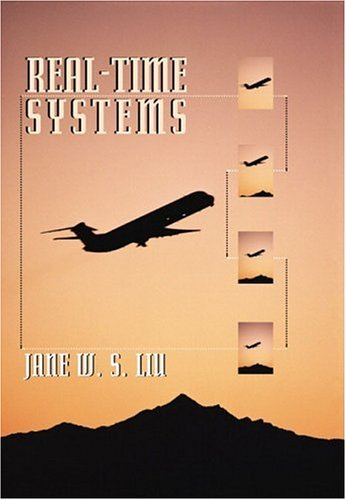
\includegraphics[scale=0.25]{pics/p2.jpg}
  \end{center}

   \begin{itemize}
  \item by Jane Liu, 2000
  \item {\it ``The job $J_l$ executes at its inherited 
    priority until it releases $R$; at that time, the 
    priority of $J_l$ returns to its priority 
    at the time when it acquires the resource $R$.''}\medskip
  \item \small gives pseudo code and totally bogus data structures  
  \item \small interesting part is ``{\it left as an exercise}''
  \end{itemize}

  \end{frame}
%%%%%%%%%%%%%%%%%%%%%%%%%%%%%%%%%%%%%%%%%%%%%%%%%%%%%%%%%%%%%%%%%%  
     
%%%%%%%%%%%%%%%%%%%%%%%%%%%%%%%%%%%%%%%%%%%%%%%%%%%%%%%%%%%%%%%%%%
  \begin{frame}[c]

  \begin{center}
  
\includegraphics[scale=0.15]{pics/p1.jpg}
  \end{center}

  \begin{itemize}
  \item by Laplante and Ovaska, 2011 (\$113.76)
  \item \it ``when $[$the task$]$ exits the critical section that
        caused the block, it reverts to the priority it had
        when it entered that section'' 
  \end{itemize}

  \end{frame}
%%%%%%%%%%%%%%%%%%%%%%%%%%%%%%%%%%%%%%%%%%%%%%%%%%%%%%%%%%%%%%%%%%  
  
%%%%%%%%%%%%%%%%%%%%%%%%%%%%%%%%%%%%%%%%%%%%%%%%%%%%%%%%%%%%%%%%%%
  \begin{frame}[c]

  \begin{center}
  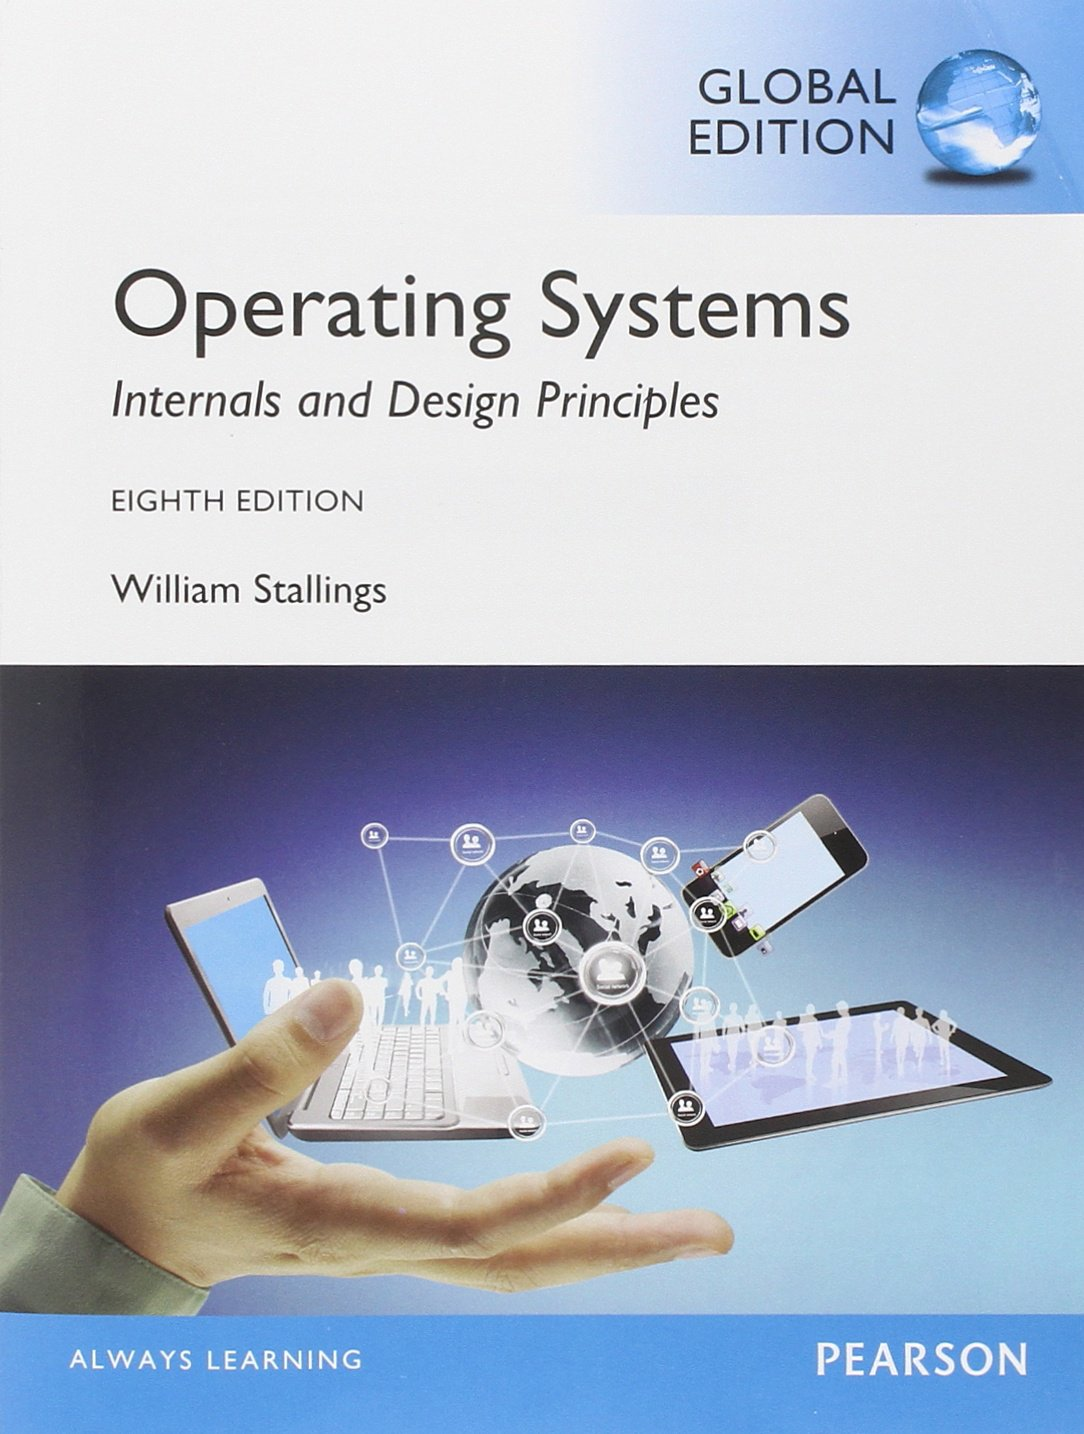
\includegraphics[scale=0.22]{pics/p5.jpg}
  \end{center}

  \begin{itemize}
  \item by Silberschatz, Galvin and Gagne (9th edition, 2013)
  \item \it ``Upon releasing the
  lock, the $[$low-priority$]$ thread will revert to its original
  priority.''
  \end{itemize}

  \end{frame}
%%%%%%%%%%%%%%%%%%%%%%%%%%%%%%%%%%%%%%%%%%%%%%%%%%%%%%%%%%%%%%%%%%  
    
  
%%%%%%%%%%%%%%%%%%%%%%%%%%%%%%%%%%%%%%%%%%%%%%%%%%%%%%%%%%%%%%%%%%
  \begin{frame}[c]
  \frametitle{Priority Scheduling}

  \begin{itemize}
  \item a scheduling algorithm that is widely used in real-time operating systems
  \item has been ``proved'' correct by hand in a paper in 1990
  \item but this algorithm turned out to be incorrect, despite its ``proof''\bigskip\pause
  
  \item we (generalised) the algorithm and then {\bf really} proved that it is correct	
  \item we implemented this algorithm in a small OS called PINTOS (used for teaching at Stanford)
  \item our implementation was faster than their reference implementation
  \end{itemize}

  \end{frame}
%%%%%%%%%%%%%%%%%%%%%%%%%%%%%%%%%%%%%%%%%%%%%%%%%%%%%%%%%%%%%%%%%%  
   

%%%%%%%%%%%%%%%%%%%%%%%%%%%%%%%%%%%%%%%%%%%%%%%%%%%%%%%%%%%%%%%%%%
  \begin{frame}[c]
  \frametitle{Lessons Learned}

  \begin{itemize}
  \item our proof-technique is adapted from security 
  protocols\bigskip
 
  \item do not venture outside your field of expertise 
  
\includegraphics[scale=0.03]{pics/smiley.jpg}
  \bigskip

  \item we solved the single-processor case; the multi-processor 
  case: no idea!
  \end{itemize}

  \end{frame}
%%%%%%%%%%%%%%%%%%%%%%%%%%%%%%%%%%%%%%%%%%%%%%%%%%%%%%%%%%%%%%%%%%  

%%%%%%%%%%%%%%%%%%%%%%%%%%%%%%%%%%%%%%%%%%%%%%%%%%%%%%%%%%%%%%%%%%
\begin{frame}[c]
\frametitle{Regular Expressions}


\begin{textblock}{6}(2,5)
  \begin{tabular}{rrl@ {\hspace{13mm}}l}
  \bl{$r$} & \bl{$::=$}  & \bl{$\varnothing$}   & null\\
           & \bl{$\mid$} & \bl{$\epsilon$}      & empty string\\
           & \bl{$\mid$} & \bl{$c$}             & character\\
           & \bl{$\mid$} & \bl{$r_1 \cdot r_2$} & sequence\\
           & \bl{$\mid$} & \bl{$r_1 + r_2$}     & alternative / choice\\
           & \bl{$\mid$} & \bl{$r^*$}           & star (zero or more)\\
  \end{tabular}
  \end{textblock}
  
\end{frame}
%%%%%%%%%%%%%%%%%%%%%%%%%%%%%%%%%%%%%%%%%%%%%%%%%%%%%%%%%%%%%%%%%%   

%%%%%%%%%%%%%%%%%%%%%%%%%%%%%%%%%%%%%%%%%%%%%%%%%%%%%%%%%%%%%%%%%%
\begin{frame}[c]
\frametitle{\begin{tabular}{c}The Derivative of a Rexp\end{tabular}}

\large
If \bl{$r$} matches the string \bl{$c\!::\!s$}, what is a regular 
expression that matches just \bl{$s$}?\bigskip\bigskip\bigskip\bigskip

\small
\bl{$der\,c\,r$} gives the answer, Brzozowski (1964), Owens (2005)
``\ldots have been lost in the sands of time\ldots''
\end{frame}
%%%%%%%%%%%%%%%%%%%%%%%%%%%%%%%%%%%%%%%%%%%%%%%%%%%%%%%%%%%%%%%%%%   

%%%%%%%%%%%%%%%%%%%%%%%%%%%%%%%%%%%%%%%%%%%%%%%%%%%%%%%%%%%%%%%%%%
\begin{frame}[c]
\frametitle{}


\ldots{}whether a regular expression can match the empty string:
\begin{center}
\begin{tabular}{@ {}l@ {\hspace{2mm}}c@ {\hspace{2mm}}l@ {}}
\bl{$nullable(\varnothing)$}      & \bl{$\dn$} & \bl{$false$}\\
\bl{$nullable(\epsilon)$}           & \bl{$\dn$} &  \bl{$true$}\\
\bl{$nullable (c)$}                    & \bl{$\dn$} &  \bl{$false$}\\
\bl{$nullable (r_1 + r_2)$}       & \bl{$\dn$} &  \bl{$nullable(r_1) \vee nullable(r_2)$} \\ 
\bl{$nullable (r_1 \cdot r_2)$} & \bl{$\dn$} &  \bl{$nullable(r_1) \wedge nullable(r_2)$} \\
\bl{$nullable (r^*)$}                 & \bl{$\dn$} & \bl{$true$} \\
\end{tabular}
\end{center}

\end{frame}
%%%%%%%%%%%%%%%%%%%%%%%%%%%%%%%%%%%%%%%%%%%%%%%%%%%%%%%%%%%%%%%%%%   

%%%%%%%%%%%%%%%%%%%%%%%%%%%%%%%%%%%%%%%%%%%%%%%%%%%%%%%%%%%%%%%%%%
\begin{frame}[c]
\frametitle{\begin{tabular}{c}The Derivative of a Rexp\end{tabular}}

\begin{center}
\begin{tabular}{@ {}l@ {\hspace{2mm}}c@ {\hspace{2mm}}l@ {\hspace{-10mm}}l@ {}}
  \bl{$der\, c\, (\varnothing)$}      & \bl{$\dn$} & \bl{$\varnothing$} & \\
  \bl{$der\, c\, (\epsilon)$}           & \bl{$\dn$} & \bl{$\varnothing$} & \\
  \bl{$der\, c\, (d)$}                     & \bl{$\dn$} & \bl{if $c = d$ then $\epsilon$ else $\varnothing$} & \\
  \bl{$der\, c\, (r_1 + r_2)$}        & \bl{$\dn$} & \bl{$der\, c\, r_1 + der\, c\, r_2$} & \\
  \bl{$der\, c\, (r_1 \cdot r_2)$}  & \bl{$\dn$}  & \bl{if $nullable (r_1)$}\\
  & & \bl{then $(der\,c\,r_1) \cdot r_2 + der\, c\, r_2$}\\ 
  & & \bl{else $(der\, c\, r_1) \cdot r_2$}\\
  \bl{$der\, c\, (r^*)$}          & \bl{$\dn$} & \bl{$(der\,c\,r) \cdot (r^*)$} &\medskip\\\pause

  \bl{$\textit{ders}\, []\, r$}     & \bl{$\dn$} & \bl{$r$} & \\
  \bl{$\textit{ders}\, (c\!::\!s)\, r$} & \bl{$\dn$} & \bl{$\textit{ders}\,s\,(der\,c\,r)$} & \\
  \end{tabular}
\end{center}

\end{frame}
%%%%%%%%%%%%%%%%%%%%%%%%%%%%%%%%%%%%%%%%%%%%%%%%%%%%%%%%%%%%%%%%%%   

%%%%%%%%%%%%%%%%%%%%%%%%%%%%%%%%%%%%%%%%%%%%%%%%%%%%%%%%%%%%%%%%%%
\begin{frame}[c]
\frametitle{\begin{tabular}{c}\bl{$({\tt a}?)^n \cdot {\tt a}^n$}\end{tabular}}

\begin{center}
\begin{tikzpicture}
\begin{axis}[
    xlabel={\pcode{a}s},
    ylabel={time in secs},
    enlargelimits=false,
    xtick={0,200,...,1000},
    xmax=1000,
    ytick={0,5,...,30},
    scaled ticks=false,
    axis lines=left,
    width=9.5cm,
    height=7cm, 
    legend entries={Python,Ruby,Scala V1,Scala V2},  
    legend pos=north west,
    legend cell align=left  
]
\addplot[blue,mark=*, mark options={fill=white}] 
  table {data/re-python.data};
\addplot[brown,mark=pentagon*, mark options={fill=white}] 
  table {data/re-ruby.data};  
\addplot[red,mark=triangle*,mark options={fill=white}] 
  table {data/re1.data};  
\addplot[green,mark=square*,mark options={fill=white}] 
  table {data/re2b.data};
\end{axis}
\end{tikzpicture}
\end{center}

\end{frame}
%%%%%%%%%%%%%%%%%%%%%%%%%%%%%%%%%%%%%%%%%%%%%%%%%%%%%%%%%%%%%%%%%%   

%%%%%%%%%%%%%%%%%%%%%%%%%%%%%%%%%%%%%%%%%%%%%%%%%%%%%%%%%%%%%%%%%%
\begin{frame}[t]
\frametitle{\begin{tabular}{c}\bl{$({\tt a}?)^n \cdot {\tt a}^n$}\end{tabular}}

\begin{center}
\begin{tikzpicture}
\begin{axis}[
    xlabel={\pcode{a}s},
    ylabel={time in secs},
    enlargelimits=false,
    xtick={0,3000,...,12000},
    xmax=12000,
    ymax=35,
    ytick={0,5,...,30},
    scaled ticks=false,
    axis lines=left,
    width=9cm,
    height=7cm
]
\addplot[green,mark=square*,mark options={fill=white}] table {data/re2b.data};
\addplot[black,mark=square*,mark options={fill=white}] table {data/re3.data};
\end{axis}
\end{tikzpicture}
\end{center}

\end{frame}
%%%%%%%%%%%%%%%%%%%%%%%%%%%%%%%%%%%%%%%%%%%%%%%%%%%%%%%%%%%%%%%%%%   

%%%%%%%%%%%%%%%%%%%%%%%%%%%%%%%%%%%%%%%%%%%%%%%%%%%%%%%%%%%%%%%%%%
\begin{frame}[c]
\frametitle{Correctness}

It is a relative easy exercise in a theorem prover:

\begin{center}
\bl{$matches(r, s)$}  if and only if  \bl{$s \in L(r)$} 
\end{center}\bigskip

\small
\bl{$matches(r, s) \dn nullable(ders(r, s))$}

\end{frame}
%%%%%%%%%%%%%%%%%%%%%%%%%%%%%%%%%%%%%%%%%%%%%%%%%%%%%%%%%%%%%%%%%%   

%%%%%%%%%%%%%%%%%%%%%%%%%%%%%%%%%%%%%%%%%%%%%%%%%%%%%%%%%%%%%%%%%%
\begin{frame}[c]
\frametitle{POSIX Regex Matching}

Two rules:

\begin{itemize}
\item Longest match rule (``maximal munch rule''): The 
longest initial substring matched by any regular expression 
is taken as the next token.

\begin{center}
\bl{$\texttt{\Grid{iffoo\VS bla}}$}
\end{center}\medskip

\item Rule priority:
For a particular longest initial substring, the first regular
expression that can match determines the token.

\begin{center}
\bl{$\texttt{\Grid{if\VS bla}}$}
\end{center}
\end{itemize}\bigskip\pause

\small
\hfill Kuklewicz: most POSIX matchers are buggy\\
\footnotesize
\hfill \url{http://www.haskell.org/haskellwiki/Regex_Posix}

\end{frame}
%%%%%%%%%%%%%%%%%%%%%%%%%%%%%%%%%%%%%%%%%%%%%%%%%%%%%%%%%%%%%%%%%% 

%%%%%%%%%%%%%%%%%%%%%%%%%%%%%%%%%%%%%%%%%%%%%%%%%%%%%%%%%%%%%%%%%%
\begin{frame}[c]
\frametitle{POSIX Regex Matching}

\begin{itemize}

\item Sulzmann \& Lu came up with a beautiful
idea for how to extend the simple regular expression 
matcher to POSIX matching/lexing (FLOPS 2014)\bigskip\bigskip\bigskip

\begin{tabular}{@{\hspace{4cm}}c@{}}
  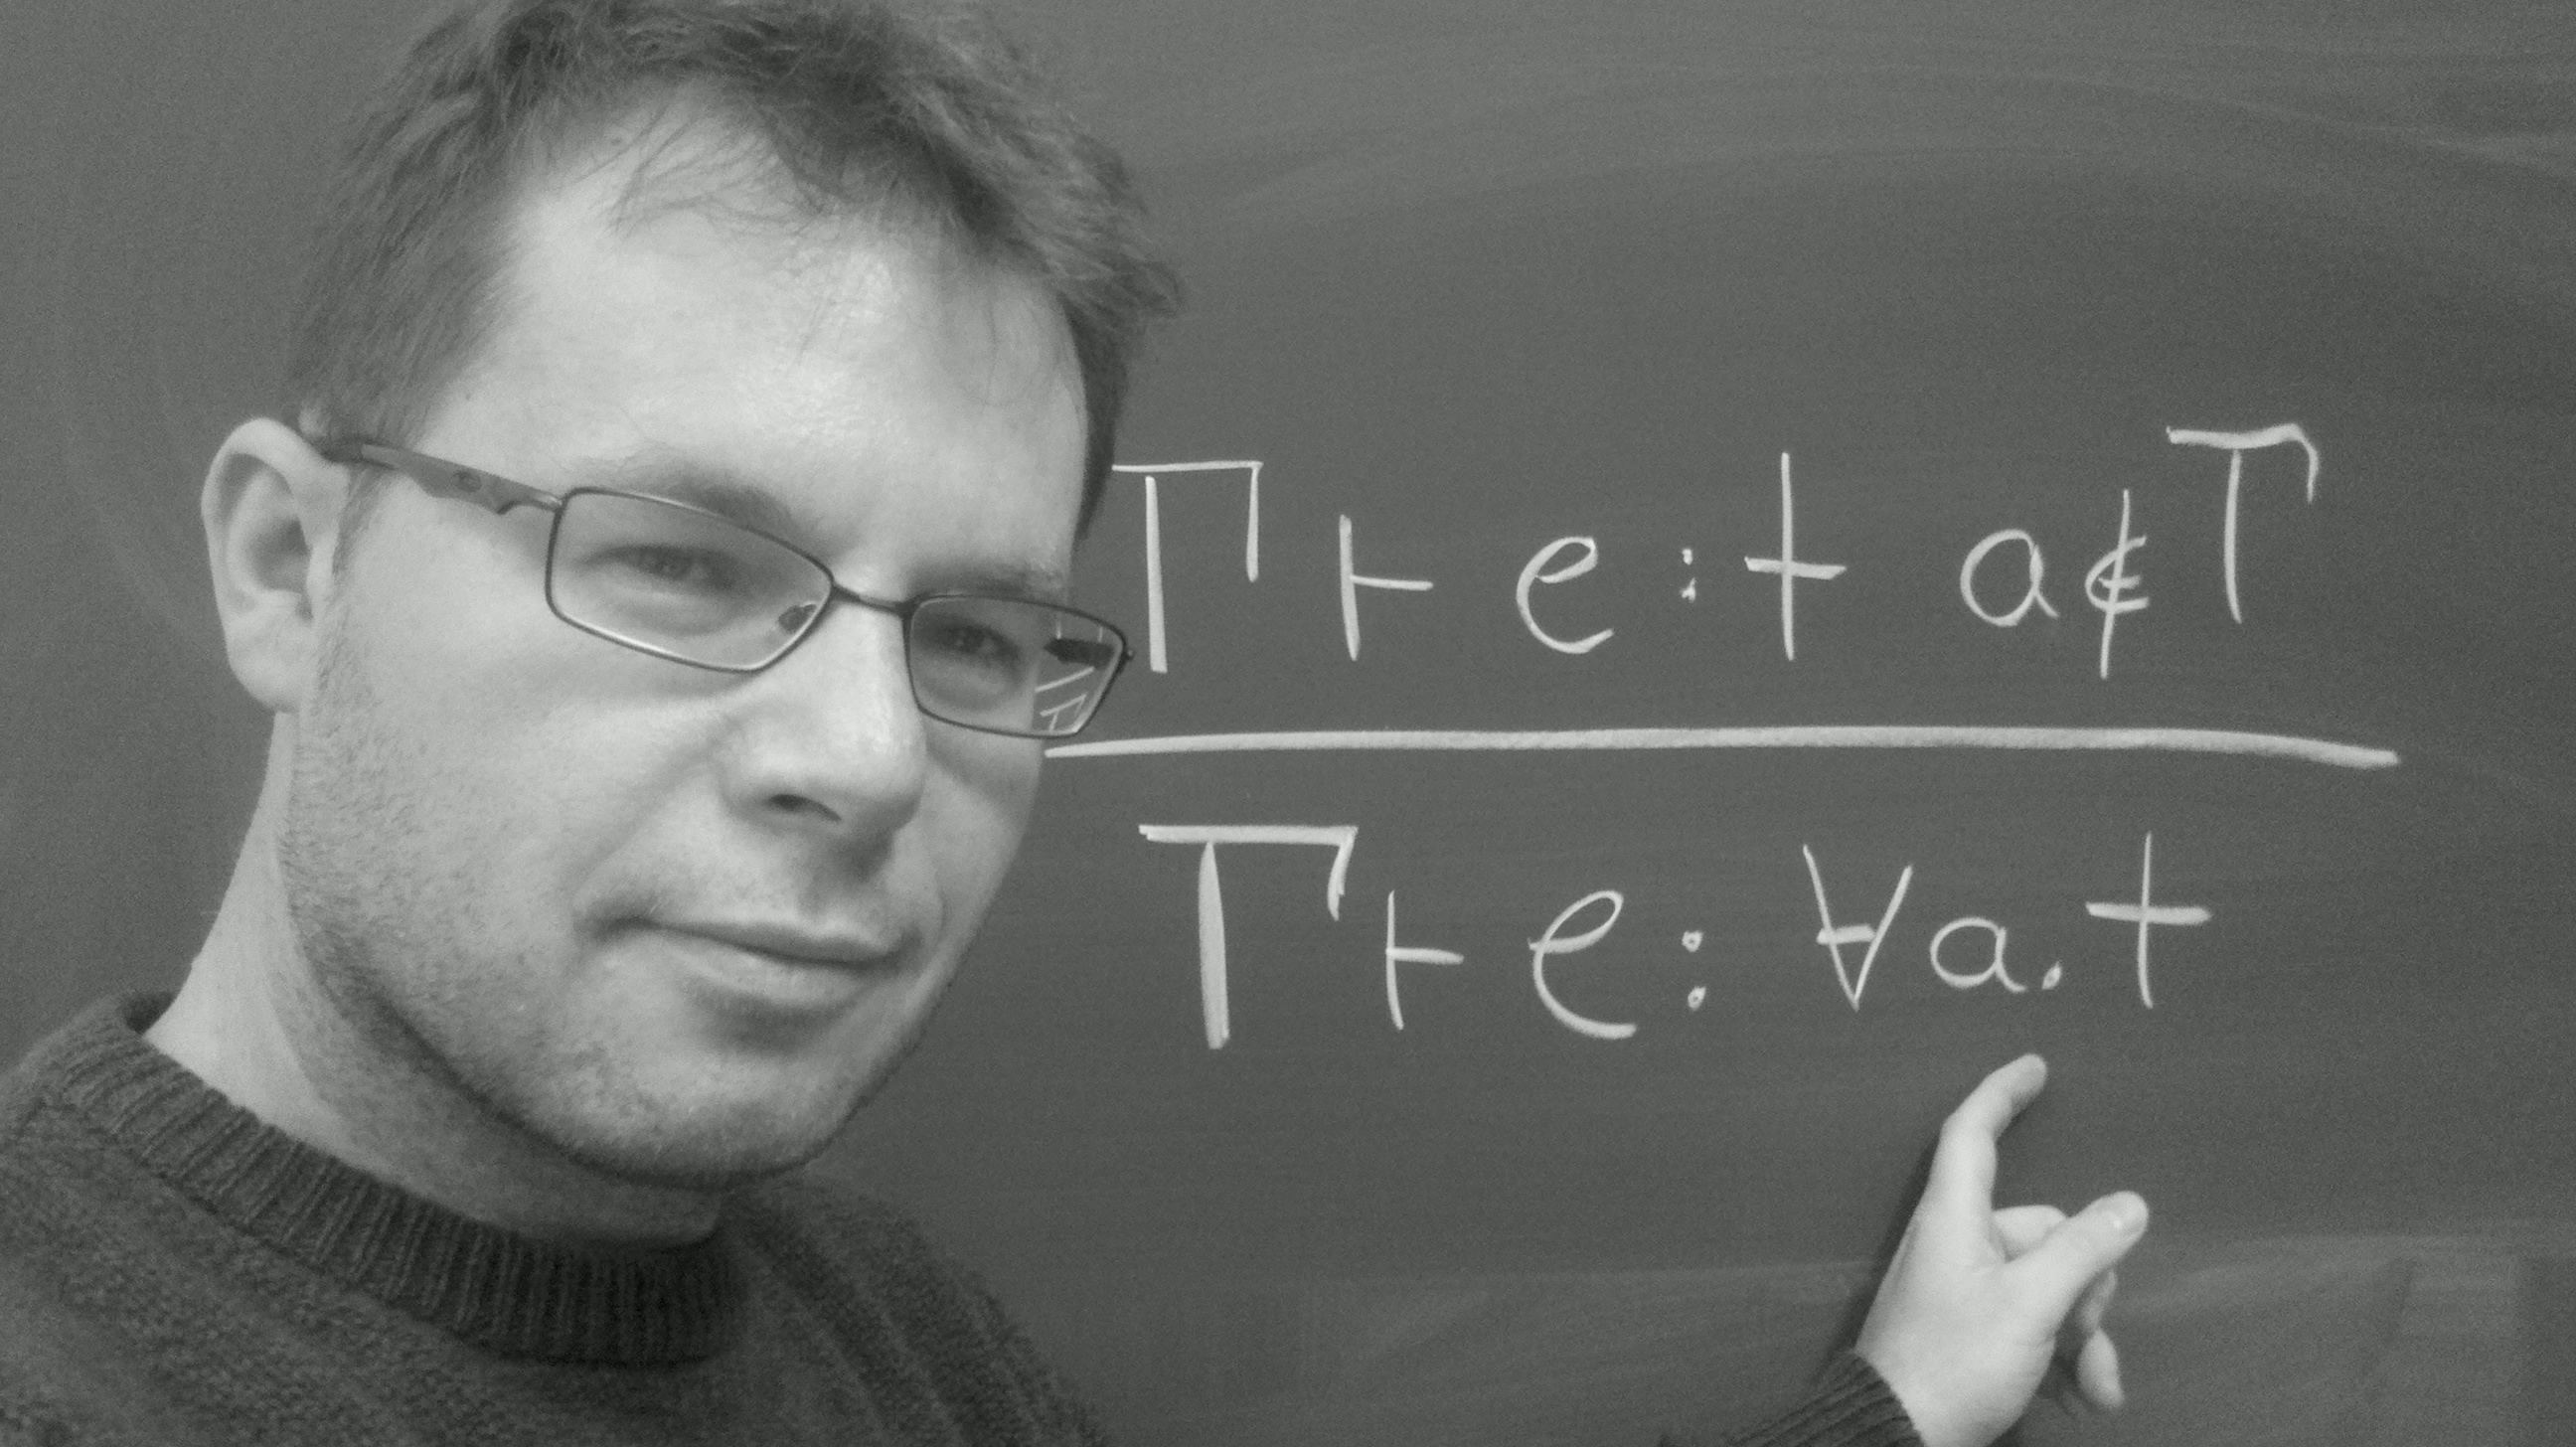
\includegraphics[scale=0.14]{pics/sulzmann.jpg}\\[-2mm]
  \hspace{0cm}\footnotesize Martin Sulzmann
\end{tabular}\bigskip\bigskip

\item the idea: define an inverse operation to the derivatives
\end{itemize}



\end{frame}
%%%%%%%%%%%%%%%%%%%%%%%%%%%%%%%%%%%%%%%%%%%%%%%%%%%%%%%%%%%%%%%%%% 


%%%%%%%%%%%%%%%%%%%%%%%%%%%%%%%%%%%%%%%%%%%%%%%%%%%%%%%%%%%%%%%%%%
\begin{frame}[c]
\frametitle{Regexes and Values}

Regular expressions and their corresponding values:

\begin{center}
\begin{columns}
\begin{column}{3cm}
\begin{tabular}{@{}rrl@{}}
  \bl{$r$} & \bl{$::=$}  & \bl{$\varnothing$}\\
           & \bl{$\mid$} & \bl{$\epsilon$}   \\
           & \bl{$\mid$} & \bl{$c$}          \\
           & \bl{$\mid$} & \bl{$r_1 \cdot r_2$}\\
           & \bl{$\mid$} & \bl{$r_1 + r_2$}   \\
  \\
           & \bl{$\mid$} & \bl{$r^*$}         \\
  \\
  \end{tabular}
\end{column}
\begin{column}{3cm}
\begin{tabular}{@{\hspace{-7mm}}rrl@{}}
  \bl{$v$} & \bl{$::=$}  & \\
           &             & \bl{$Empty$}   \\
           & \bl{$\mid$} & \bl{$Char(c)$}          \\
           & \bl{$\mid$} & \bl{$Seq(v_1,v_2)$}\\
           & \bl{$\mid$} & \bl{$Left(v)$}   \\
           & \bl{$\mid$} & \bl{$Right(v)$}  \\
           & \bl{$\mid$} & \bl{$[]$}      \\
           & \bl{$\mid$} & \bl{$[v_1,\ldots\,v_n]$} \\
  \end{tabular}
\end{column}
\end{columns}
\end{center}\pause

There is also a notion of a string behind a value: \bl{$|v|$}

\end{frame}
%%%%%%%%%%%%%%%%%%%%%%%%%%%%%%%%%%%%%%%%%%%%%%%%%%%%%%%%%%%%%%%%%%   


%%%%%%%%%%%%%%%%%%%%%%%%%%%%%%%%%%%%%%%%%%%%%%%%%%%%%%%%%%%%%%%%%%
\begin{frame}[c]
\frametitle{Sulzmann \& Lu Matcher}

We want to match the string \bl{$abc$} using \bl{$r_1$}:

\begin{center}
\begin{tikzpicture}[scale=2,node distance=1.3cm,every node/.style={minimum size=8mm}]
\node (r1)  {\bl{$r_1$}};
\node (r2) [right=of r1] {\bl{$r_2$}};
\draw[->,line width=1mm]  (r1) -- (r2) node[above,midway] {\bl{$der\,a$}};\pause
\node (r3) [right=of r2] {\bl{$r_3$}};
\draw[->,line width=1mm]  (r2) -- (r3) node[above,midway] {\bl{$der\,b$}};\pause
\node (r4) [right=of r3] {\bl{$r_4$}};
\draw[->,line width=1mm]  (r3) -- (r4) node[above,midway] {\bl{$der\,c$}};\pause
\draw (r4) node[anchor=west] {\;\raisebox{3mm}{\bl{$\;\;nullable?$}}};\pause
\node (v4) [below=of r4] {\bl{$v_4$}};
\draw[->,line width=1mm]  (r4) -- (v4);\pause
\node (v3) [left=of v4] {\bl{$v_3$}};
\draw[->,line width=1mm]  (v4) -- (v3) node[below,midway] {\bl{$inj\,c$}};\pause
\node (v2) [left=of v3] {\bl{$v_2$}};
\draw[->,line width=1mm]  (v3) -- (v2) node[below,midway] {\bl{$inj\,b$}};\pause
\node (v1) [left=of v2] {\bl{$v_1$}};
\draw[->,line width=1mm]  (v2) -- (v1) node[below,midway] {\bl{$inj\,a$}};\pause
\draw[->,line width=0.5mm]  (r3) -- (v3);
\draw[->,line width=0.5mm]  (r2) -- (v2);
\draw[->,line width=0.5mm]  (r1) -- (v1);
\draw (r4) node[anchor=north west] {\;\raisebox{-8mm}{\bl{$mkeps$}}};
\end{tikzpicture}
\end{center}

\end{frame}
%%%%%%%%%%%%%%%%%%%%%%%%%%%%%%%%%%%%%%%%%%%%%%%%%%%%%%%%%%%%%%%%%%   

%%%%%%%%%%%%%%%%%%%%%%%%%%%%%%%%%%%%%%%%%%%%%%%%%%%%%%%%%%%%%%%%%%
\begin{frame}[t,squeeze]
\frametitle{Sulzmann \& Lu Paper}

\begin{itemize}
\item I have no doubt the algorithm is correct --- 
  the problem, I do not believe their proof.

  \begin{center}
  \begin{bubble}[10cm]\small
  ``How could I miss this? Well, I was rather careless when 
  stating this Lemma :)\smallskip
 
  Great example how formal machine checked proofs (and 
  proof assistants) can help to spot flawed reasoning steps.''
  \end{bubble}
  \end{center}\pause
  
  \begin{center}
  \begin{bubble}[10cm]\small
  ``Well, I don't think there's any flaw. The issue is how to 
  come up with a mechanical proof. In my world mathematical 
  proof $=$ mechanical proof doesn't necessarily hold.''
  \end{bubble}
  \end{center}\pause
  
\end{itemize}

  \only<3>{%
  \begin{textblock}{11}(1,4.4)
  \begin{center}
  \begin{bubble}[10.9cm]\small\centering
  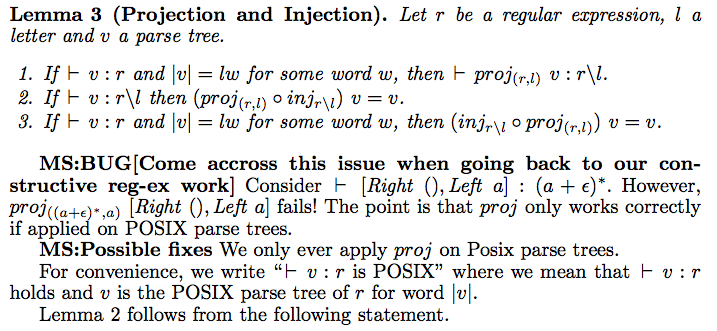
\includegraphics[scale=0.37]{pics/msbug.png}
  \end{bubble}
  \end{center}
  \end{textblock}}
  

\end{frame}
%%%%%%%%%%%%%%%%%%%%%%%%%%%%%%%%%%%%%%%%%%%%%%%%%%%%%%%%%%%%%%%%%% 

%%%%%%%%%%%%%%%%%%%%%%%%%%%%%%%%%%%%%%%%%%%%%%%%%%%%%%%%%%%%%%%%%%
\begin{frame}[c]
\frametitle{\begin{tabular}{c}The Proof Idea\\[-1mm] by Sulzmann \& Lu
\end{tabular}}

\begin{itemize}
\item introduce an inductively defined ordering relation 
\bl{$v \succ_r v'$} which captures the idea of POSIX matching

\item the algorithm returns the maximum of all possible
 values that are possible for a regular expression.\pause
 \bigskip\small
 
\item the idea is from a paper by Cardelli \& Frisch about 
greedy matching (greedy $=$ preferring instant gratification to delayed
repletion):

\item e.g.~given \bl{$(a + (b + ab))^*$} and string \bl{$ab$}

\begin{center}
\begin{tabular}{ll}
greedy: & \bl{$[Left(a), Right(Left(b)]$}\\
POSIX:  & \bl{$[Right(Right(a, b)))]$}  
\end{tabular}
\end{center} 
\end{itemize}

\end{frame}
%%%%%%%%%%%%%%%%%%%%%%%%%%%%%%%%%%%%%%%%%%%%%%%%%%%%%%%%%%%%%%%%%%%%%%%%%%%%

%%%%%%%%%%%%%%%%%%%%%%%%%%%%%%%%%%%%%%%%%%%%%%%%%%%%%%%%%%%%%%%%%%
\begin{frame}[c]
\frametitle{}
\centering


\bl{\infer{\vdash Empty : \epsilon}{}}\hspace{15mm}
\bl{\infer{\vdash Char(c): c}{}}\bigskip

\bl{\infer{\vdash Seq(v_1, v_2) : r_1\cdot r_2}{\vdash v_1 : r_1 \quad \vdash v_2 : r_2}}
\bigskip

\bl{\infer{\vdash Left(v) : r_1 + r_2}{\vdash v : r_1}}\hspace{15mm}
\bl{\infer{\vdash Right(v): r_1 + r_2}{\vdash v : r_2}}\bigskip

\bl{\infer{\vdash [] : r^*}{}}\hspace{15mm}
\bl{\infer{\vdash [v_1,\ldots, v_n] : r^*}
          {\vdash v_1 : r \quad\ldots\quad \vdash v_n : r}}

\end{frame}
%%%%%%%%%%%%%%%%%%%%%%%%%%%%%%%%%%%%%%%%%%%%%%%%%%%%%%%%%%%%%%%%%% 

%%%%%%%%%%%%%%%%%%%%%%%%%%%%%%%%%%%%%%%%%%%%%%%%%%%%%%%%%%%%%%%%%%
\begin{frame}<1>[c]
\frametitle{}
\small

%\begin{tabular}{@{}lll@{}}
%\bl{$POSIX(v, r)$} & \bl{$\dn$} & \bl{$\vdash v : r$}\\ 
% & &   \bl{$\wedge \;\;(\forall v'.\;\; \vdash v' : r \,\wedge\, |v'| = |v| 
%     \Rightarrow v \succ_{\alert<2>{r}} v')$}
%\end{tabular}\bigskip\bigskip\bigskip


\centering

%\bl{\infer{Seq(v_1, v_2) \succ_{\alert<2>{r_1\cdot r_2}} Seq(v'_1, v'_2)}
%   {v_1 = v'_1 \quad v_2 \succ_{\alert<2>{r_2}} v'_2}}\hspace{3mm}
%\bl{\infer{Seq(v_1, v_2) \succ_{\alert<2>{r_1\cdot r_2}} Seq(v'_1, v'_2)}
%   {v_1 \not= v'_1 \quad v_1 \succ_{\alert<2>{r_1}} v'_1}}
%\bigskip

%\bl{\infer{Left(v) \succ_{\alert<2>{r_1 + r_2}} Left(v')}
%          {v \succ_{\alert<2>{r_1}} v'}}\hspace{15mm}
%\bl{\infer{Right(v) \succ_{\alert<2>{r_1 + r_2}} Right(v')}
%          {v \succ_{\alert<2>{r_2}} v'}}\bigskip\medskip

%\bl{\infer{Left(v) \succ_{\alert<2>{r_1 + r_2}} Right(v')}
%          {length |v|  \ge length |v'|}}\hspace{15mm}
%\bl{\infer{Right(v) \succ_{\alert<2>{r_1 + r_2}} Left(v')}
%          {length |v| >  length |v'|}}\bigskip

%\bl{$\big\ldots$}

\end{frame}
%%%%%%%%%%%%%%%%%%%%%%%%%%%%%%%%%%%%%%%%%%%%%%%%%%%%%%%%%%%%%%%%%% 


%%%%%%%%%%%%%%%%%%%%%%%%%%%%%%%%%%%%%%%%%%%%%%%%%%%%%%%%%%%%%%%%%%
\begin{frame}[c]
\frametitle{Problems}

\begin{itemize}
\item Sulzmann: \ldots Let's assume \bl{$v$} is not 
    a $POSIX$ value, then there must be another one
    \ldots contradiction.\bigskip\pause

\item Exists?

\begin{center}
\bl{$L(r) \not= \varnothing \;\Rightarrow\; POSIX(v, r)$}
\end{center}\bigskip\bigskip\pause

\item in the sequence case, the induction hypotheses require
\bl{$|v_1| = |v'_1|$} and \bl{$|v_2| = |v'_2|$}, 
but you only know

\begin{center}
\bl{$|v_1| \;@\; |v_2| = |v'_1| \;@\; |v'_2|$}
\end{center}\pause\small

\item although one begins with the assumption that the two 
values have the same flattening, this cannot be maintained 
as one descends into the induction (alternative, sequence)
\end{itemize}

\end{frame}
%%%%%%%%%%%%%%%%%%%%%%%%%%%%%%%%%%%%%%%%%%%%%%%%%%%%%%%%%%%%%%%%%% 

%%%%%%%%%%%%%%%%%%%%%%%%%%%%%%%%%%%%%%%%%%%%%%%%%%%%%%%%%%%%%%%%%%
\begin{frame}[c]
\frametitle{Our Solution}

\begin{itemize}
\item direct definition of what a POSIX value is, using
\bl{$s \in r \to v$}:

\begin{center}
\bl{\infer{[] \in \epsilon \to Empty}{}}\hspace{15mm}
\bl{\infer{c \in c \to Char(c)}{}}\bigskip\medskip

\bl{\infer{s \in r_1 + r_2 \to Left(v)}
          {s \in r_1 \to v}}\hspace{10mm}
\bl{\infer{s \in r_1 + r_2 \to Right(v)}
          {s \in r_2 \to v & s \not\in L(r_1)}}\bigskip\medskip

\bl{\infer{s_1 @ s_2 \in r_1 \cdot r_2 \to Seq(v_1, v_2)}
          {\small\begin{array}{l}
           s_1 \in r_1 \to v_1 \\
           s_2 \in r_2 \to v_2 \\
           \neg(\exists s_3\,s_4.\; s_3 \not= []
           \wedge s_3 @ s_4 = s_2 \wedge
           s_1 @ s_3 \in L(r_1) \wedge
           s_4 \in L(r_2))
           \end{array}}}
           
\bl{\ldots}           
\end{center}
\end{itemize}

\end{frame}
%%%%%%%%%%%%%%%%%%%%%%%%%%%%%%%%%%%%%%%%%%%%%%%%%%%%%%%%%%%%%%%%%%%%
\begin{frame}[t]
  \frametitle{\Large\begin{tabular}{@{}c@{}}Pencil-and-Paper Proofs\\[-1mm] 
  in CS are normally incorrect\end{tabular}}

\begin{itemize}
\item case in point, in one of Roy's proofs he made the 
incorrect inference

\begin{center}
if \bl{$\forall s.\; |v_2| \alert{\not}\in L(der\,c\,r_1) \cdot s$}
then \bl{$\forall s.\; c\,|v_2| \alert{\not}\in L(r_1) \cdot s$}
\end{center}\bigskip

while 

\begin{center}
if \bl{$\forall s.\; |v_2| \in L(der\,c\,r_1) \cdot s$}
then \bl{$\forall s.\; c\,|v_2| \in L(r_1) \cdot s$}
\end{center}

is correct

\end{itemize}


\begin{textblock}{11}(12,11)
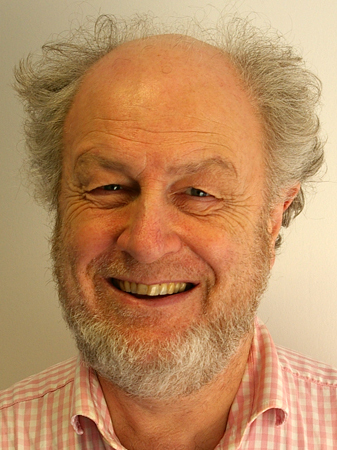
\includegraphics[scale=0.15]{pics/roy.jpg}
\end{textblock}
\end{frame}
%%%%%%%%%%%%%%%%%%%%%%%%%%%%%%%%%%%%%%%%%%%%%%%%%%%%%%%%%%%
  \begin{frame}[c]
  \frametitle{Proofs in Math~vs.~in CS}
  
  \alert{\bf My theory on why CS-proofs are often buggy}
  \\[-10mm]\mbox{}
  
  \begin{center}
  \begin{tabular}{@{}cc@{}}
  \begin{tabular}{@{}p{5.6cm}} 
  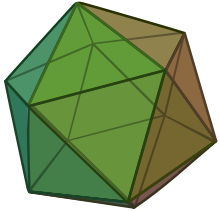
\includegraphics[scale=0.43]{pics/icosahedron.png}\\[2mm] 
  {\bf Math}: \\
  \raggedright\small
  in math, ``objects'' can be ``looked'' at from all 
  ``angles'';\\\smallskip 
  non-trivial proofs, but it seems
  difficult to make mistakes
  \end{tabular} &
  \begin{tabular}{p{5cm}} 
  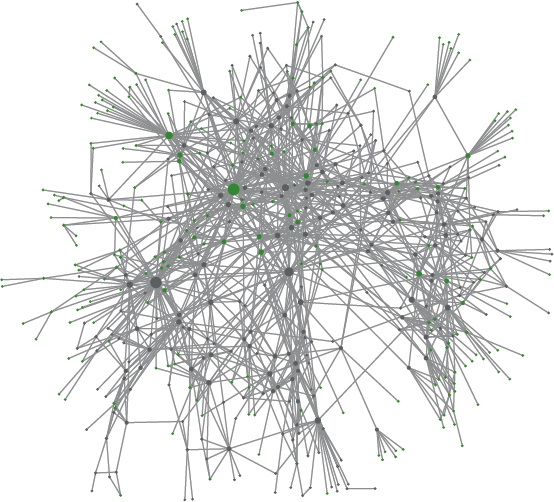
\includegraphics[scale=0.2]{pics/sel4callgraph.jpg}\\[3mm]
  \raggedright
  {\bf Code in CS}: \\
  \raggedright\small
  the call-graph of the seL4 microkernel OS;\\\smallskip 
  easy to make mistakes\\ \mbox{}\\
  \end{tabular}
  \end{tabular}
  \end{center}

  \end{frame}
%%%%%%%%%%%%%%%%%%%%%%%%%%%%%%%%%%%%%%%%%%%%%%%%%%%%%%%%%%%


%%%%%%%%%%%%%%%%%%%%%%%%%%%%%%%%%%%%%%%%%%%%%%%%%%%%%%%%%%%%%%%%%%
\begin{frame}[c]
\frametitle{Conclusion}

\begin{itemize}
\item we strengthened the POSIX definition of Sulzmann \& Lu
  in order to get the inductions through, his proof
  contained small gaps but had also fundamental flaws\bigskip

\item its a nice exercise for theorem proving
\item some optimisations need to be aplied to the
 algorithm in order to become fast enough
\item can be used for lexing, small little functional 
 program
\end{itemize}

\end{frame}
%%%%%%%%%%%%%%%%%%%%%%%%%%%%%%%%%%%%%%%%%%%%%%%%%%%%%%%%%%%%%%%%%% 


%%%%%%%%%%%%%%%%%%%%%%%%%%%%%%%%%%%%%%%%%%%%%%%%%%%%%%%%%%%%%%%%%%
  \begin{frame}[b]
  \frametitle{
  \begin{tabular}{c}
  \mbox{}\\[13mm]
  \alert{\Large Thank you very much again}\\
  \alert{\Large for the invitation!}\\
  \alert{\Large Questions?}
  \end{tabular}}

  \end{frame}
%%%%%%%%%%%%%%%%%%%%%%%%%%%%%%%%%%%%%%%%%%%%%%%%%%%%%%%%%%%%%%%%%%     

\end{document}


%%% Local Variables:  
%%% mode: latex
%%% TeX-master: t
%%% End: 

